\documentclass[12pt]{article}
\usepackage{graphicx}
\usepackage{booktabs}
\usepackage[font=footnotesize,skip=5pt]{caption}
\usepackage[font=scriptsize,skip=0pt]{subcaption}
\usepackage{amsmath}
\usepackage{amsfonts}
\usepackage{amssymb}
\usepackage{lscape}
\usepackage{psfrag}
\usepackage[usenames]{color}
\usepackage{bbm}
\usepackage[update]{epstopdf}
\usepackage[bookmarks,pdfstartview=FitH,a4paper,pdfborder={0 0 0}]{hyperref}
\usepackage{verbatim}
\usepackage{listings}
\usepackage{textcomp}
\usepackage{course}
\usepackage{fancyhdr}
\usepackage{multirow}
\pagestyle{fancy}
\usepackage{tikz}
\usepackage{bm}
\usepackage{float}
%\usepackage{subfig}

\renewcommand{\sectionmark}[1]{\markboth{#1}{#1}}
\renewcommand{\subsectionmark}[1]{\markright{#1}}

\newtheorem{theorem}{Theorem}
\DeclareMathOperator{\Var}{Var}
\DeclareMathOperator{\Bias}{Bias}

\graphicspath{ {../../Images/} }
\usepackage[backend=biber, style=bwl-FU, sorting=nyt]{biblatex}
\addbibresource{bib.bib}

\fancyhf{}
\fancyhead[RO]{\nouppercase{\footnotesize\sc\leftmark\ \hrulefill\ \thepage}}
%\fancyhead[RE]{\nouppercase{\footnotesize\sc\thepage\ \hrulefill\ }}
\renewcommand{\headrulewidth}{0pt}

\makeatletter
\def\cleardoublepage{\clearpage\if@twoside \ifodd\c@page\else%
\hbox{}%
\thispagestyle{empty}%
\clearpage%
\if@twocolumn\hbox{}\clearpage\fi\fi\fi}
\makeatother


\renewcommand{\topfraction}{0.9}  % max fraction of floats at top
\renewcommand{\bottomfraction}{0.8} % max fraction of floats at bottom
% Parameters for TEXT pages (not float pages):
\setcounter{topnumber}{2}
\setcounter{bottomnumber}{2}
\setcounter{totalnumber}{4}            % 2 may work better
\setcounter{dbltopnumber}{2}           % for 2-column pages
\renewcommand{\dbltopfraction}{0.9}    % fit big float above 2-col. text
\renewcommand{\textfraction}{0.07}     % allow minimal text w. figs
% Parameters for FLOAT pages (not text pages):
\renewcommand{\floatpagefraction}{0.7}  % require fuller float pages
% N.B.: floatpagefraction MUST be less than topfraction !!
\renewcommand{\dblfloatpagefraction}{0.7} % require fuller float pages

\sloppy

\widowpenalty=10000
\clubpenalty=10000

\edef\today{%\number\day\
\ifcase\month\or
January\or February\or March\or April\or May\or June\or July\or
August\or September\or October\or November\or December\fi\ \number\year}
\title{\vspace*{40.0mm}
  \bf Report on project about regression
         \vspace*{20.0mm} \\
  %\vspace{-20mm}\framebox{DRAFT VERSION}\vspace{20mm} \\
  \Large\bf Statistical Data Analysis 
  
 
  
  Project 3 \vspace*{20.0mm}
  \vspace*{40.0mm}}
\author{Mitja Mandić}
\date{ May 2022}

\begin{document}

\begin{figure}
  \parbox[t]{125mm}{
    \vspace*{6mm}
    \scriptsize\sf           DEPARTMENT OF MATHEMATICS \\
    \scriptsize\sf           FACULTY OF SCIENCE\\
    \scriptsize\sf           KU LEUVEN}
  \parbox[t]{40mm}{
    \begin{flushright}
      
\includegraphics[height=15mm]{../images/logo.eps.pdf}
    \end{flushright}}
\end{figure}

\maketitle
\thispagestyle{empty}
\raggedbottom

\cleardoublepage
\pagenumbering{roman}
\setcounter{tocdepth}{2}
%\tableofcontents
\pagenumbering{arabic}

\section{Introduction}
For this assignment we switch from dataset on canteloupe melons to analysing the $\text{CO}_{2}$ emissions in grams per kilometer
of cars from 2000 to 2013. As usual we select a random subsample of the data we do our study on, this time of size 500.

\section{Full model analysis}\label{fullModel}
Firstly, we draw a correlation matrix to check for potential multicollinearity in the data. Note that we also had to remove categorical
variables \texttt{euro\_standard, fuel\_type} and \texttt{transmission\_type} from the data to do perform the calculations.

\begin{figure}[!h]
  \centering
  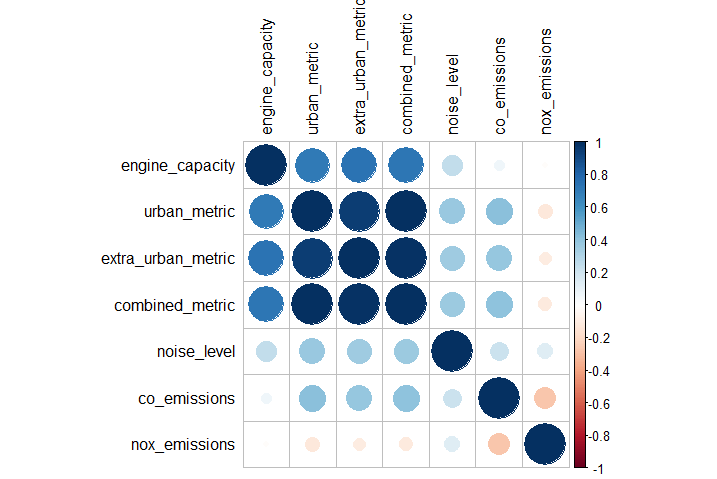
\includegraphics[width=0.5\textwidth]{project3/corrplot.png}
  \caption{Correlation matrix of numeric predictors}
  \label{fig:corrplot}
\end{figure}
In figure \ref{fig:corrplot} we see that there is in fact some significant correlation between ``metric'' variables and engine capacity.
Since combined metric is a weighted average of urban and extra-urban metric correlation between them is expected. Intuition also
tells us that the larger engines consume more fuel, so corrleation to this variable is also not surprising. Calculating the correlation
with the response variable, previously mentioned covariates are the most correlated with it. Below all values are presented.

\begin{verbatim}
co2  engine_capacity urban_metric extra_urban_metric combined_metric 
1.00 0.75            0.98         0.97               0.99            
noise_level co_emissions nox_emissions 
0.40        0.34         0.02
\end{verbatim}

We move on to fit the full model, meaning we include all the data as our covariates. While most of the coefficients in the model are
statistically significant, \texttt{euro\_standard4, urban\_metric, extra\_urban\_metric, noise\_level} and \texttt{co\_emissions} all have p-values above 0.05.
\verbatiminput{cars.full.output.txt}


\begin{figure}
  \centering
  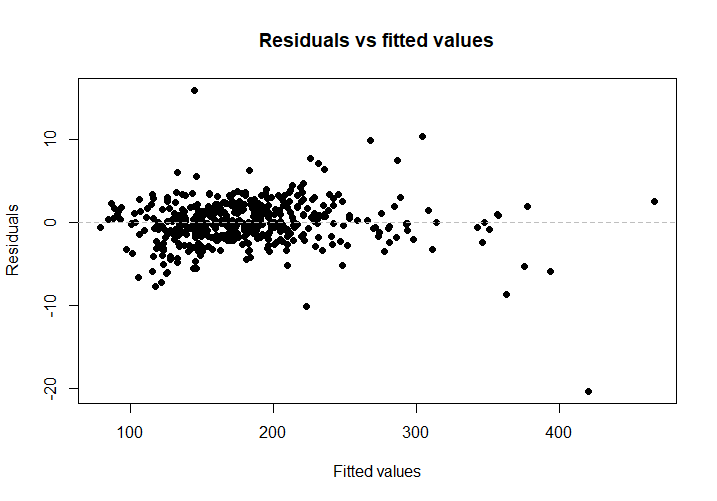
\includegraphics[width=0.5\textwidth]{project3/resVsFit_full.png}
  \caption{Residuals versus fitted value of the full model}
  \label{fig:resVsFit_full}
\end{figure}


Even though a few variables are non-significant, the linear model assumptions are satisfied. The mean of errors is zero
and their variance does not differ across the data. From the plot of errors versus fitted values we see that in the largest datacloud no trends
are appearing. Fewer cars have very large fitted values of their $\text{CO}_2$ emissions and their residuals very a bit more.

Some outliers are present.

\begin{figure}[h]
  \begin{subfigure}[b]{0.5\linewidth}
      \centering
      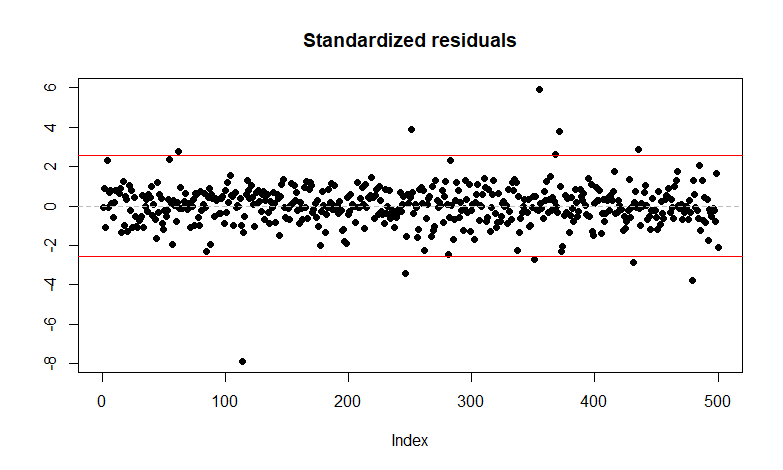
\includegraphics[width=\textwidth]{project3/cars.full.res.png}
      \caption{Plot of standardized residuals}
      \label{fig:cars.full.res}
  \end{subfigure}%
  %
  \begin{subfigure}[b]{0.5\linewidth}
      \centering
   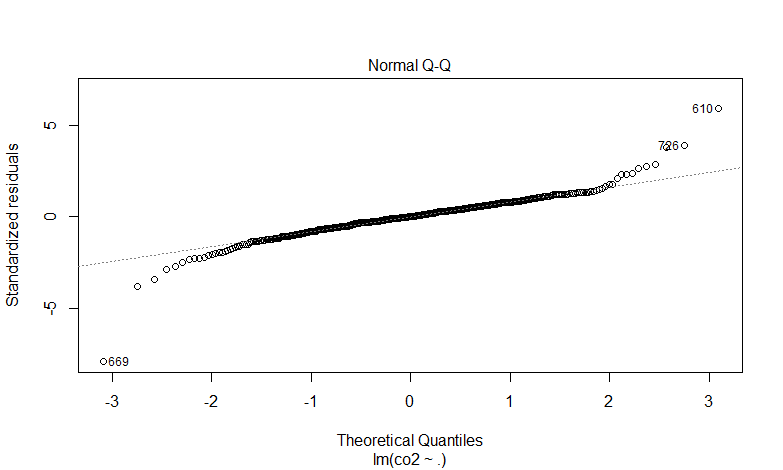
\includegraphics[width=\textwidth]{project3/QQ_cars.full.res.png}
   \caption{Normal Q-Q plot of standardised resiudals}\label{fig:QQ_cars.full}
  \end{subfigure}%
 \caption{Investigating behaviour of residuals of the full model}
\end{figure}

From the Q-Q plot in figure \ref{fig:QQ_cars.full} we can conclude that the residuals normally distributed, as the majority fall on the 
diagonal line with some deviation towards the tails, with the three most notable outliers being Maserati Spyder (669 -- very fancy sports car),
Daewoo cars Matiz (610 -- small family car from South-Korea) and Volkswagen Touareg (label 726).
This way we also confirm that Gauss-Markov conditions hold.

\section{Transforming the response variable}
\subsection{Box-Cox transformation}
In the following section we turn our attention to potentially improving our model by transforming the response variable. We start off
by applying the Box-Cox transformation, for which we obtain $\lambda = -0.14.$ This however does not yield satisfactoty results. The
adjusted $R^2$ value remains high at 0.951, however the residuals do not exhibit trends of normal distribution. Several more outliers 
appear in the negative direction. The Q-Q plot shows heavier tails than in the model without a transformation and plotting
resiudals versus fitted values shows a quadratic trend.
\begin{figure}[h]
  \centering
  \textbf{Box-Cox transformed response}
  \begin{subfigure}[b]{0.5\linewidth}
      \centering
      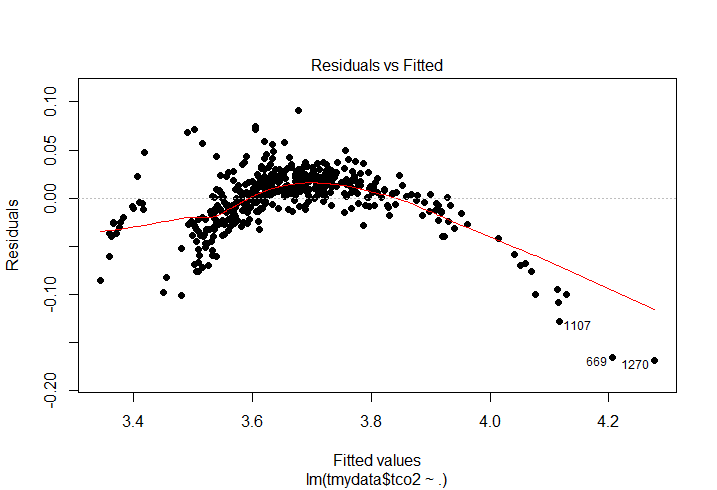
\includegraphics[width=\textwidth]{project3/resVsFit_BoxCox.png}
      \caption{Plot of standardized residuals \\ for the Box-Cox transformed response}
      \label{fig:resVsFit_BoxCox}
  \end{subfigure}%
  %
  \begin{subfigure}[b]{0.5\linewidth}
      \centering
   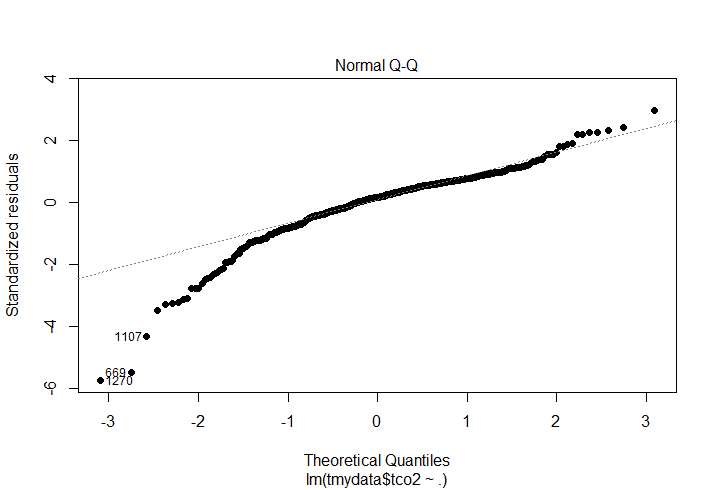
\includegraphics[width=\textwidth]{project3/QQ_BoxCox.png}
   \caption{Normal Q-Q plot of standardised resiudals for \\the Box-Cox transformed variable}\label{fig:QQ_BoxCox}
  \end{subfigure}%
 \caption{Investigating behaviour of residuals of the full model with Box-Cox transformed response variable}
 \label{fig:BoxCox}
\end{figure}

\subsection{Logarithm transformation}
We proceed with a logarithm of the response variable. The conclusions are fairly similar to the transformation with $\lambda=-0.14,$ which
is not completely surprising as the logarithm is simply a Box-Cox with parameter zero. As the plots look alike to those in figure \ref{fig:BoxCox}
we do not include them here. We do not use the logarithm to transform the response
either.

\subsection{Square root}
The last option we check here is the square root. Once again we find that the transformation does not improve the fit. Residuals versus
fitted value plot in figure \ref{fig:resVsFit_sqrt} exhibits a quadratic trend, and especially error's the lower tail is much heavier
than in the normal distribution, as seen in \ref{fig:QQ_sqrt}.

The MSE of all models with a transformed response is lower compared to the original model, while also their adjusted $R^2$ remaining
relatively high (lowest with Box-Cox transformation at 0.95). However, since their residuals behave in a strange manner any further inference
with these models would be invalid. Therefore we conclude, that no transformation is needed for our data.

\begin{figure}[!h]
  \centering
  \textbf{Square root of the response}
  \begin{subfigure}[b]{0.5\linewidth}
      \centering
      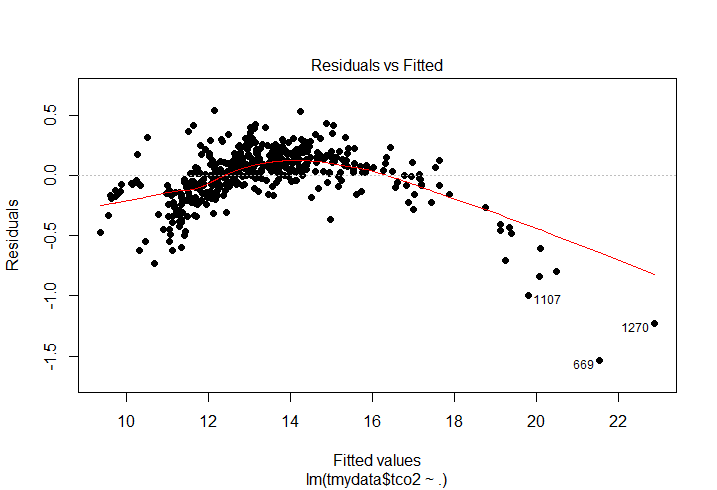
\includegraphics[width=\textwidth]{project3/resVsFit_sqrt.png}
      \caption{Plot of standardized residuals for the square root of \\ the response}
      \label{fig:resVsFit_sqrt}
  \end{subfigure}%
  %
  \begin{subfigure}[b]{0.5\linewidth}
      \centering
   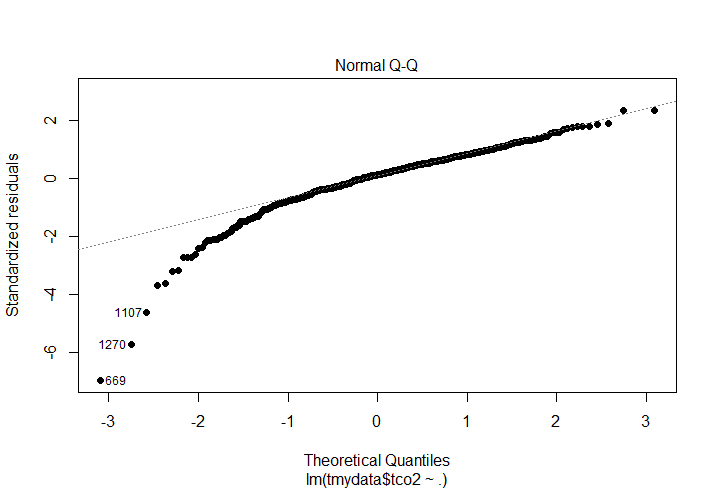
\includegraphics[width=\textwidth]{project3/QQ_sqrt.png}
   \caption{Normal Q-Q plot of standardised resiudals for the square root of the response}\label{fig:QQ_sqrt}
  \end{subfigure}%
 \caption{Investigating behaviour of residuals of the full model with square root of the response variable}
\end{figure}



\section{Variable selection} \label{varSec}
As mentioned in section \ref{fullModel} some variables in the full model appear to be statistically insignificant. We will now try
to improve our model by eliminating them. 

First we try to remove all variables with too high p-value, that is \texttt{urban\_metric, extra\_urban\_metric, noise\_level} 
and \texttt{co\_emissions}, simultaneously (\texttt{euro\_standard4} is 
part of a categorical variable). In this model all coefficients except for those corresponding to \texttt{euro\_standard4} and 
\texttt{euro\_standard6} are significant. Applying the F-test to check whether this can be done however rejects this hypothesis with
a p-value of 0.0013.

This changes after  we add \texttt{extra\_urban\_metric} to our model. That way we do not reject the null that coefficients are
zero and all covariates (except \texttt{euro\_standard4} and \texttt{euro\_standard6}) are significant. The adjusted $R^2$ value
remains very high at 0.9975 (compared to 0.9976 in the original model). Residuals behave appropriately and in fact rather similarly
to the full model. Since omitted variables do not seem to add anything to the model we continue our project with the 
sparser one, now conisting of: euro standard, transmission type, engine capacity, fuel type, extra urban metric, combined metric and 
$\text{NO}_\text{x}$ emissions.

\subsection{Can we remove \texttt{euro\_standard} from the model?}
Using the \texttt{anova} function on the reduced model, which still contains the variable \texttt{euro\_standard}, we see in the results
of the partial F-test that we cannot remove this variable from our model - the p-value obtained is essentially zero. 
Looking into the results in greater detail 
we see a very large p-value for \texttt{euro\_standard4}, which implies that the slope for these cars is statistically the same as the 
baseline, which is \texttt{euro\_standard3}. This is not the case for cars with engines of higher standards, as both of those have p-values
below the 0.05. Therefore we cannot remove all slopes corresponding to \texttt{euro\_standard} from our model simultaneously.

\section{Confidence and prediction intervals}
Continuing to work with the reduced model introduced in the previous section \ref{varSec}, we construct the prediction and confidence interval
answering questions 5 and 6.

\subsection{Confidence interval for $\beta_1$}
Following the mentioned model, $\beta_1$ corresponds to the coefficient in front of \texttt{euro\_standard4}. The 95\% confidence
interval is then $[-0.698,0.961].$
We see that 0 is a possible option for this value, however removing all slopes related to \texttt{euro\_standard} is still not possible 
as confidence intervals for other values do not include 0.

\subsection{Prediction interval}
Here we construct a 99\% prediction interval for a car with the following specifications: \texttt{euro\_standard} = 4, \texttt{transmission\_type}
= ``Manual'', \texttt{engine\_capacity} = 2196, \texttt{fuel\_type} = ``Petrol'', \texttt{urban\_metric} =
9.2, \texttt{extra\_urban\_metric} = 5.6, \texttt{combined\_metric} = 6.9, \texttt{noise\_level} = 72, \texttt{co\_emissions}
= 273.5, \texttt{nox\_emissions} = 43. 

Prediction interval for its $\text{CO}_2$ emissions in grams per kilometer is $[156.35,170.48].$

\end{document}